%--------------------------------------------------------
%| CGAL Manual : tpm.tex
%|
%| Soon to be split into User and Reference Manuals
%--------------------------------------------------------
%| Specification of topological planar map
%|
%| 31 Mar 2000  - Shai Hirsch, 
%|    changes for the 31/3/2000 deadline
%|
%| Version  1.1 - Iddo Hanniel
%|    changes after lutz's comments in MPI
%| Version  1.0 - Iddo Hanniel
%|    
%--------------------------------------------------------

\def\Ipe#1{\def\IPEfile{#1}\input{#1}}

\renewcommand{\Re}{{\rm I\!\hspace{-0.025em} R}}
\newcommand{\normal}[1]{\eta_{#1}}
\newenvironment{dfn}{{\vspace*{1ex} \noindent \bf Definition }}{\vspace*{1ex}}
\newcommand{\bigdef}[2]{\index{#1}\begin{dfn} {\rm #2} \end{dfn}}
\newenvironment{proof}{{\em Proof:}}{\hfill{\hfill\rule{2mm}{2mm}}}

\newcommand{\comment}[1]{{\sf * #1 *}}
\newcommand{\ncomment}[1]{\noindent {\sf * #1 * }}

\newcommand{\intsupplanes}{P} 
\def\C{{\cal C}}
\def\G{{\cal G}}
\def\F{{\cal F}}
\def\I{{\cal I}}
\def\U{{\cal U}}
\def\M{{\cal M}}
\def\eps{{\varepsilon}}
\def\bd{{\partial}}
\def\dm{{\cal D}}
\newcommand{\Section}[1]{Section~{\protect\ref{#1}}}
\newcommand{\Chapter}[1]{Chapter~{\protect\ref{#1}}}

% restores original settings for \parskip and \parindent
\ccParDims

\chapter{Topological Maps}
\label{I1_ChapterTopologicalMap}
\minitoc

% +=============================================================+
\section{Introduction}
\label{TPM_sec:intro}
   The topological map (\ccc{Topological_map<Dcel>}) is a {\em
   combinatorial} structure with no geometric information. Therefore,
   it can also be used as a base class for deriving geometric
   subdivisions (e.g, 2D planar maps) with different geometries (e.g,
   on a sphere or torus). 

\section{Basic Terms and Software Design}
   The class is parametrized with the \ccc{Dcel} type which should
   model the \ccc{TopologicalMapDcel} concept. The \ccc{Dcel} (Doubly
   Connected Edge List) is the underlying combinatorial data structure
   (also know as the halfedge data structure).

   The \ccc{Planar_map_2<Dcel,Traits>} class
   (Chapter~\ref{I1_ChapterPlanarMap}) is derived from the
   \ccc{Topological_map<Dcel>} class and it describes an embedding of
   a topological map in the Euclidean plane.  This chapter and Chapter
   \ref{I1_ChapterPlanarMap} describe the \ccc{Topological_map} class
   and the \ccc{Planar_map} class respectively. These classes supply
   the ability to maintain subdivisions of the plane induced by
   collections of curves. In this chapter we introduce the
   \ccc{topological map}. In this section we briefly review the
   concepts underlying the data structures described in the following
   sections as well as the functionality of \ccc{Topological_map} in a
   nutshell.

\begin{figure}
\begin{ccTexOnly}
    \centerline{
      %\includegraphics{my_face.ps}
      \Ipe{my_face.ipe}
    }
\end{ccTexOnly}
\caption{A face, an edge, and a vertex \label{fig:face}}

\begin{ccHtmlOnly}
  <P>
  <center><img border=0 src="my_face.gif" alt=" ">
  <!-- <br> A face, an edge, and a vertex -->
  </center>
\end{ccHtmlOnly}

\end{figure}

% \ccHtmlNoLinksFrom prevents Vertex from being linked to hds' vertex
\ccHtmlNoLinksFrom{
\paragraph{Topological Map, Vertex, Edge, Face:} 
}
A topological map is a graph that consists of vertices V,
edges E, faces F and an incidence relation on them. %\ccSeeAlso{Polyhedron} 
Each edge is represented by two halfedges with opposite orientations.
A {\em face} of the topological map is defined by the ordered
circular sequences 
(inner and outer) of halfedges along its boundary. 

\paragraph{Incidence:}
If a vertex $v$ is an endpoint of an edge $e$, then we say that $v$
and $e$ are {\em incident} to each other. Similarly, a face and an
edge on its boundary are incident, and a face and a vertex on its
boundary are incident (including edges and vertices that are not connected 
to the outer boundary --- see below).

\ccHtmlNoLinksFrom{
\paragraph{Halfedge, Twin, Source, Target:}
}
We consider each edge $e$ to be two-sided, representing it by two
directed {\em halfedges} \lcTex{$\vec{e}$}\lcHtml{$e$} and 
\lcTex{${\rm Twin}(\vec{e})$}\lcHtml{${\rm Twin}({e})$} 
(In other packages the twin halfedge is called $opposite$).  
A halfedge \lcTex{$\vec{e}$}\lcHtml{$e$} is an ordered pair $(u,v)$ of its endpoints, and
it is directed from $u$, the {\em source}, to $v$, the {\em target} (there 
is no need to store both in each halfedge since 
\lcTex{${\rm Target}(\vec{e}) \equiv {\rm Source}({\rm Twin}(\vec{e}))$}%
\lcHtml{${\rm Target}({e}) \equiv {\rm Source}({\rm Twin}({e}))$}).
We consider each halfedge to lie on the boundary of a single face.

%---the face lying to our left as we traverse the edge from source to target.

%We consider each edge $e$ to be two-sided, representing it by two
%directed {\em halfedges} \ccTexHtml{$\vec{e}$}{$e$} and
%\ccTexHtml{${\rm Twin}(\vec{e})$}{${\rm Twin}(e)$} (in other 
%places the twin halfedge is called $Opposite$).  
%A halfedge \ccTexHtml{$\vec{e}$}{$e$}
%is an ordered pair $(u,v)$ of its incident vertices, and
%it is directed from $u$, the {\em source}, to $v$, the {\em target} (there 
%is no need to store both in each halfedge since
%\ccTexHtml{${\rm Target}(\vec{e}) \equiv {\rm Source}({\rm Twin}(\vec{e}))$}{${\rm Target}(e) \equiv {\rm Source}({\rm Twin}(e))$}).
%We consider each halfedge to lie on the boundary of a single face.
%%---the face lying to our left as we traverse the edge from source to target.

\paragraph{Connected Component of the Boundary (CCB):}
Each connected component of the boundary of a face is %represented 
defined by a
circular list of halfedges. 
%The list of halfedges of the 
%outer boundary component of a face is oriented counterclockwise, and
%the list for each inner boundary component is oriented clockwise, see
%Figure \ref{fig:DCEL}.  
For a face $f$ of a topological map, 
we call each
connected component of the boundary of $f$ a {\em CCB}.
A {\em bounded face} has a
unique CCB that is defined to be
its outer CCB. An
{\em unbounded\/} face does not have an outer boundary.
In the topological map we have one unbounded face.
%If $f$ is
%bounded, we call its outer boundary component the outer CCB. 
Except for the outer CCB, any other
connected component of the boundary of $f$ is called a hole (or inner CCB),
every face can have none
or several holes.
We say that the holes are {\em contained\/} inside
the face.

\ccHtmlNoLinksFrom{
\paragraph{Edges around a Vertex :}
}
Every maximal set of halfedges that share the same target can be viewed 
as a circular list of halfedges ordered %clockwise  
around their target vertex.
It should be noted that the orientation of the edges around a vertex is 
opposite to that of the halfedges around a face, i.e., if edge $e2$
succeeds edge $e1$ in the order given around vertex $v$, then $e1$
succeeds $e2$ in the order given around the incident face $f$.
Unlike the convention we adopt
for \ccc{Planar_map} in Chapter~\ref{I1_ChapterPlanarMap} where the halfedges
are oriented counterclockwise around a face and clockwise around a vertex,
in the topological map the users are free to choose any other convention.

\begin{figure}
\begin{ccTexOnly}
    \centerline{
       \Ipe{dcel.ipe}
       }
\end{ccTexOnly}
\caption{Source and target vertices, and twin halfedges \label{fig:DCEL}}

\begin{ccHtmlOnly}
<P>
<center><img border=0 src="./dcel.gif" alt=" ">
<!-- <br> Source and target vertices, and twin halfedges -->
</center>
\end{ccHtmlOnly}
\end{figure}

\paragraph{Doubly Connected Edge List (DCEL):}
For a topological map, its {\em DCEL} representation consists of a
connected list of halfedges for every CCB of every face in the
subdivision, with additional incidence information that enables us to
traverse the subdivision. %In particular, for 
For each halfedge the DCEL
stores a pointer to its twin halfedge and to the next
halfedge around its incident face (see Figure~\ref{fig:DCEL}). In
addition, for each halfedge the DCEL stores a pointer to the incident
face and the target vertex.
For each face the DCEL stores a pointer to a halfedge representing
its outer-CCB and an iterator over pointers to halfedges representing
its inner-CCBs (traversing over a CCB is thus done with repetitive
calls to the next halfedge pointer).
For each vertex the DCEL stores a pointer to an incident halfedge. 
For more information about the DCEL
representation see ~\cite{bkos-cgaa-97} and Chapter~\ref{chapterHds}
on \ccStyle{Halfedge_data_structure}.
The DCEL is a low-level container class that stores the objects.
The topological map layer adds high-level functions and protection of
combinatorial validity. Iterators, handles and circulators are also
introduced in this layer (pointers are no longer visible in this layer).

In the following
specifications, we implement the subdivision by a DCEL. 
%See Section
%~\ref{DCEL_sec:req}
%for a specification of the requirements for a DCEL in our implementation.

\subsection*{Functionality}

The class \ccc{Topological_map<Dcel>} supplies the ability to maintain
a topological map. The user can insert edges in various ways and then split,
merge or remove them as well as move holes from one face to another.
The vertices, edges and faces can be traversed in a 
linear way or any other fashion mentioned above.
For a full reference of the class (i.e its associated types,
its operations, etc.) read the \ccc{Topological_map Reference Pages}\lcTex{
(\ccRefPage{Tpm_ref_intro})}.


% +=============================================================+
\section{Example Programs}
\label{TPM_sec:example}
We conclude this chapter with two example programs. The first example
demonstrates a simple construction of a \ccc{Topological_map}. The 
second example demonstrates the ease with which additional information can
be added to the \ccc{Topological_map}.

% +-------------------------------------------------------------+
\subsection{Simple Topological Map}
The example shows a simple construction of a \ccStyle{Topological_map}.
It uses the base classes for vertex, halfedge and face and demonstrates
the use of the three insertion functions.

The function \ccc{is_valid()} checks the validity of the topological map.

\ccIncludeExampleCode{Topological_map/example1.C}

The output of the program is:

\begin{verbatim}
inserting edge e1 in face interior ...map is valid.
inserting edge e2 from target vertex of e1 ...map is valid.
inserting edge e3 between target vertices of e2 and e1->twin() ...map is valid.

\end{verbatim}

%%%%%%%%%%%%%%%%%%

\subsection{Topological Map with Additional Information}
The example shows a construction of a \ccStyle{Topological_map}
with additional information in the faces. It uses inheritance from the face 
base class to add the information. 

\ccIncludeExampleCode{Topological_map/example2.C}

The output of the program is:

\begin{verbatim}
inserting e1 in face interior...
inserting e2 from vertex...
inserting e3 between vertices of e2 and e1->twin()...

setting info of the new face to 10...

unbounded face info = 0
new face info = 10
\end{verbatim}

% +-------------------------------------------------------------+

% EOF
